\chapter{Comparisons with Other Channels}
\label{chap:compare}
ATLAS has published comparisons of the released Full Run 2 results~\cite{ATL-PHYS-PUB-2021-031}, shown for the 
spin-0 resonant results in Figure \ref{fig:res-comparison} and the non-resonant results in Figure 
\ref{fig:nonres-comparison}. 
The results of this thesis for the $\bbbb$ channel are included in the resonant plot up to \SI{3}{\TeV}. The 
preliminary non-resonant results presented here are not yet included. Both figures include a comparison with the 
combined early Run 2 result~\cite{HDBS-2018-58}.

For the resonant, the \bbbb channel has the leading sensitivity above a mass of around \SI{700}{\GeV}, and 
is competitive across much of the considered range, though it has limited sensitivity at very low masses. The 
individual channels shown in general represent improvements over the early Run 2 combined result, a promising 
indicator for a large increase in sensitivity with the full Run 2 combination across channels, for which the 
\bbbb channel will be a strong contributor.

\begin{figure}[ht]
\centering
\subfloat{
		  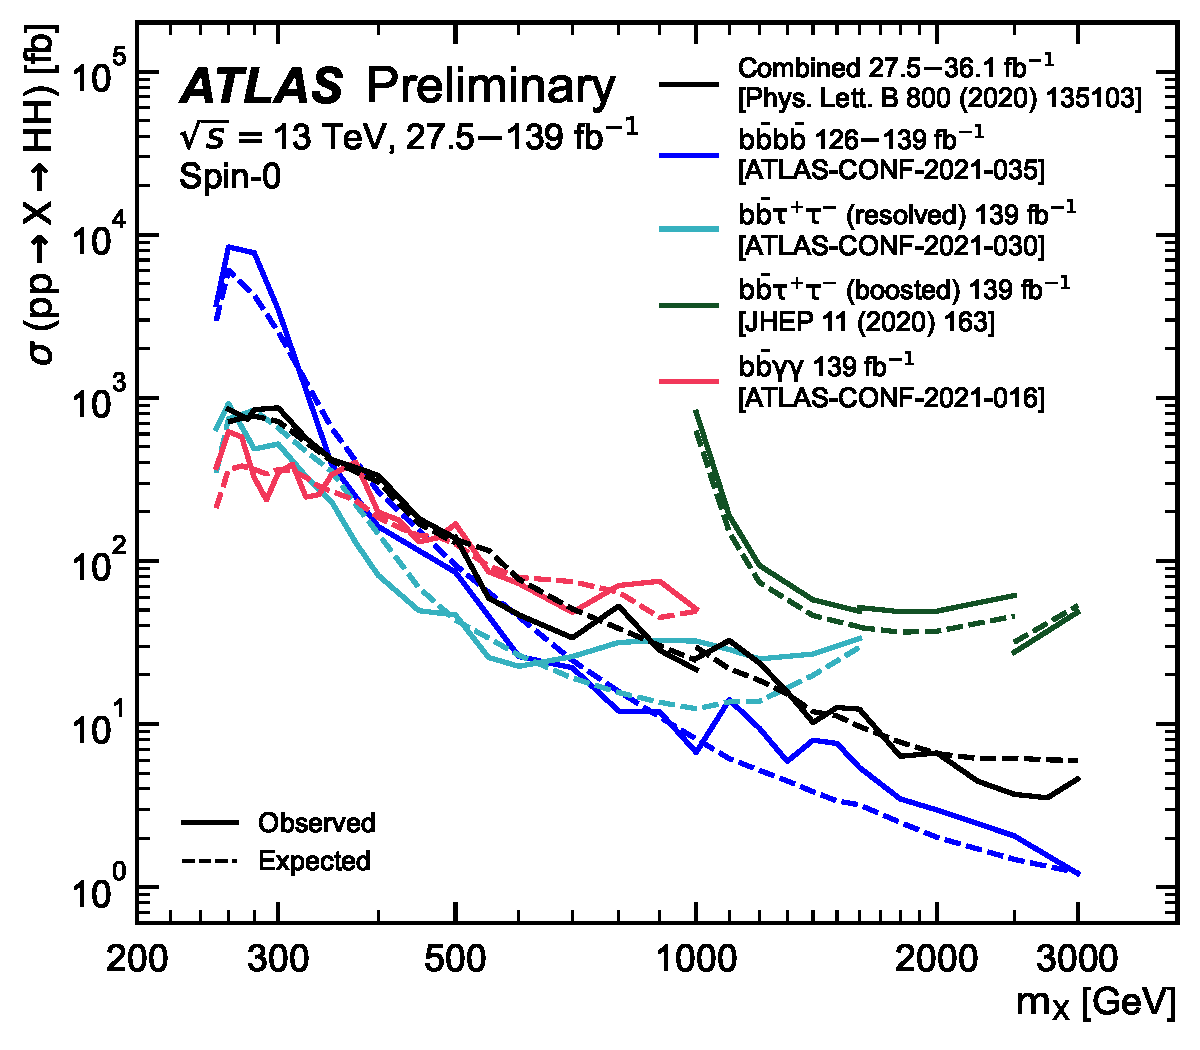
\includegraphics[width=0.8\textwidth]{figures/full-run2-summary-res.pdf}
		 }

\caption{\label{fig:res-comparison} Comparison of full Run 2 ATLAS $HH$ searches for spin-0 resonances. The \bbbb 
channel (blue) is compared with full Run 2 results from $b\bar{b}\tau^{+}\tau^{-}$ (both resolved and boosted) and  
$b\bar{b}\gamma\gamma$, as well as the combined early Run 2 results. The \bbbb channel has leading sensitivity above 
a mass of around \SI{700}{\GeV}, and is competitive with other channels across much of the mass range, demonstrating 
a strong contribution to the ATLAS $HH$ experimental results.~\cite{ATL-PHYS-PUB-2021-031}}
\end{figure}

The Standard Model non-resonant limits presented in this thesis are $4.4(5.9)$ times the Standard Model observed (expected) 
for the gluon-gluon fusion channel only. This is a significant gain on its own above the early Run 2 combined result. 
Though the leading channels presented in Figure \ref{fig:nonres-comparison} include both VBF and ggF production modes, and 
are normalized as such, the \bbbb results of this thesis can still be seen to be quite competitive, again demonstrating a 
strong contribution to the ATLAS experimental results for $HH$. Roughly estimating the combined result for full Run 2 
\bbbb, $b\bar{b}\tau^{+}\tau^{-}$, and $b\bar{b}\gamma\gamma$ yields a limit of around 2 to 3 times the Standard Model. 
Such a result sets the stage for a very exciting Run 3 -- with a projected factor of around $2\times$ increase in 
luminosity, plus any additional analysis improvements, sensitivity to $HH$ may be just on the horizon.
\begin{figure}[ht]
\centering
\subfloat{
		  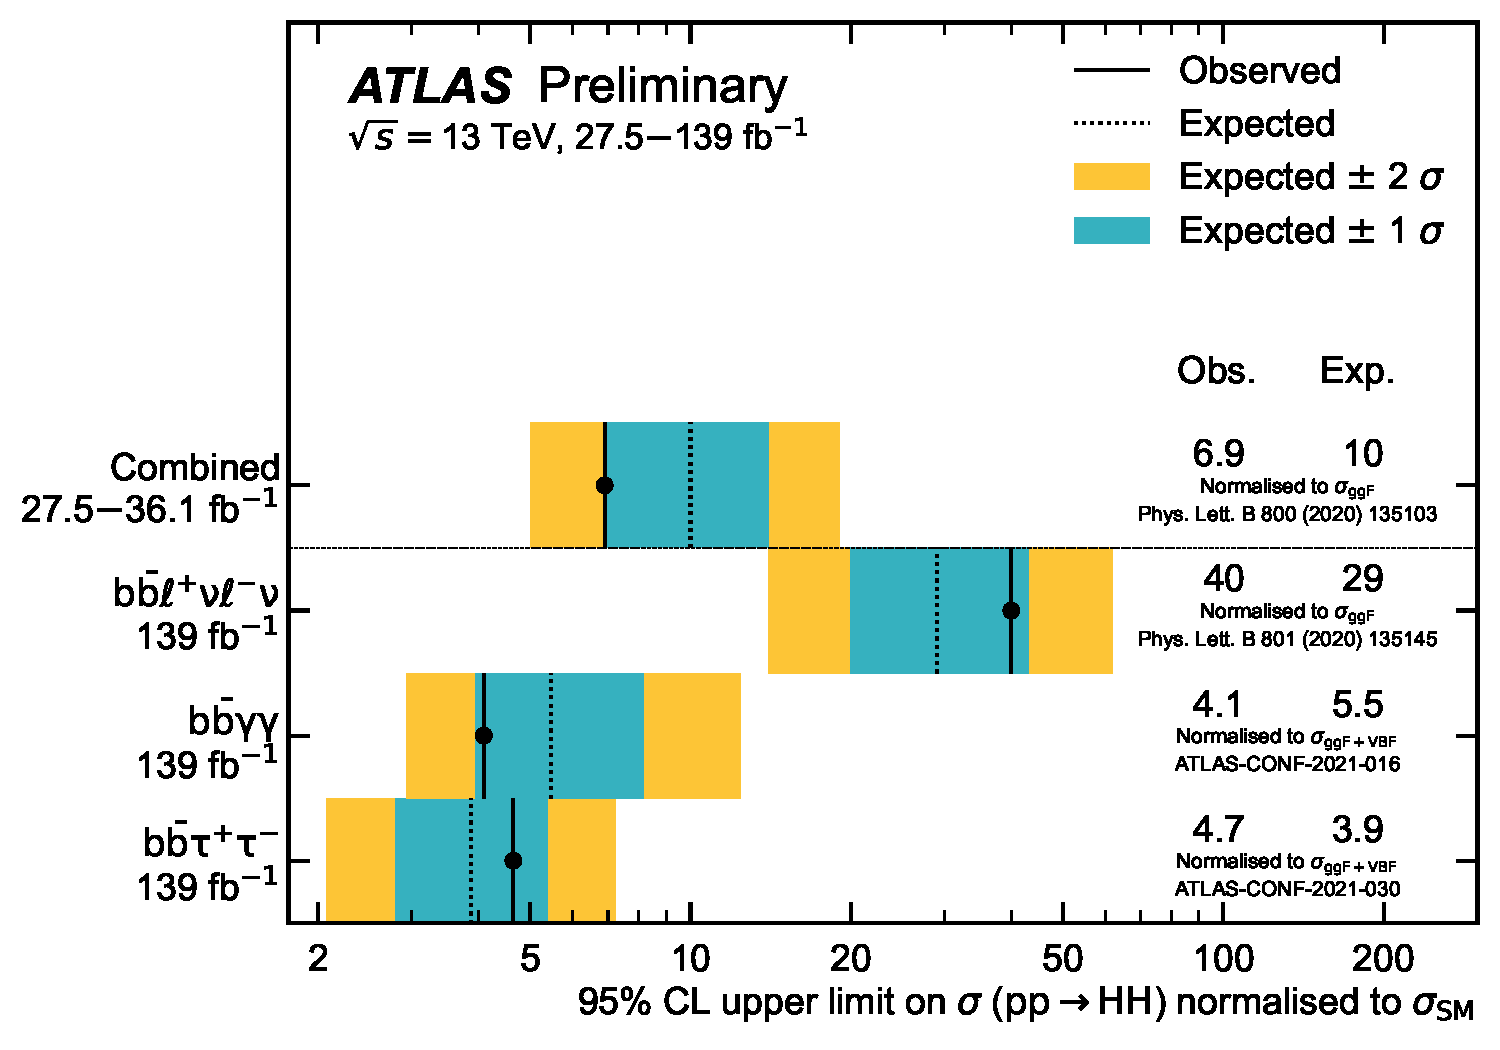
\includegraphics[width=0.8\textwidth]{figures/full-run2-summary-non-res.pdf}
		 }

\caption{\label{fig:nonres-comparison} Comparison of full Run 2 ATLAS $HH$ searches for Standard Model $HH$ production. 
The preliminary results presented in this thesis are not yet included in these results. However, the results presented 
in Table \ref{tbl:SM-HH-limits} are quite competitive with the results from $b\bar{b}\tau^{+}\tau^{-}$ and 
$b\bar{b}\gamma\gamma$, two of the ATLAS channels with leading sensitivity in the search for HH. Note that these 
results include signals produced via both gluon-gluon fusion (ggF) and vector boson fusion (VBF), and are normalized as 
such, while the results of this thesis only include (and are normalized to) ggF production ~\cite{ATL-PHYS-PUB-2021-031}}
\end{figure}